% Introduction
\chapter*{Introduction}

% Welcome to :-)
\section*{Welcome to \IzPack !}

\fbox{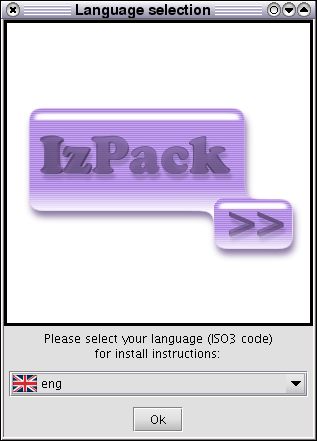
\includegraphics[scale=0.5]{img/lang-sel-splash}}
\IzPack is a tool that will help you to solve your software installation
problems. It is a \Java based software installer builder that will run
on any operating system coming with a \textit{Java Virtual Machine
(JVM)} that is compliant with the Sun JVM 1.2 or higher. Its design is
very modular and you will be able to choose how \textbf{you} want your
installer to look and you will also be able to customize it using a very
simple \textit{Application Programming Interface (API)}. Although
\IzPack is essentially a \Java only application (it can run on virtually
any operating system), it can interact in a clean way with the
underlying operating system. Native code can interact with it on a
specific platform without disturbing the operation on incompatible
operating systems. For instance, you can develop Unix-specific code that
will be silent if run on Windows. To put it in a nutshell, whereas most
of the other \Java installers force you to go their way, \IzPack will
let you go \textbf{your way}. Some respectable companies have been using
it in order to produce customized  installers for their \textsl{very}
specific needs.\\

\textit{"So, if it's so good, how much is it ?"} : well, you can get it
for free. \textbf{BUT} \IzPack is not a \textit{freeware}. It's not
\textit{free} as in \textit{"free beer"} but \textit{"free as in free
speech"}. So it's neither \textit{freeware} nor \textit{public domain}.
It is software covered by the \textsc{GNU General Public License} (GPL).
It uses the tactic of \textit{copyleft} : to make it short, you can use
it, modify it and redistribute it freely but you must also make your
modifications available to everyone whenever you publish a modified
version of a \textit{copylefted} software. You have access to the
\IzPack source code and you can modify it to make it suit your needs,
but if you publish such a modified version, you are forced to publish
the modifications you've made. \underline{That's a fair exchange of
expertise and  work}. To learn more about the GPL license and the
\textit{copyleft} principles, visit \mbox{\url{http://www.gnu.org/}}.\\

% Features
\section*{The Features}

\IzPack uses XML files to describe installations. When you make an
installer, you have a choice of panels. You can see panels as a kind of
plugin that composes the installer. For instance, a panel can choose the
installation path, the packs to install, prompt the user for a license
agreement and so on. This approach is very modular. You can also create
your own panels if you have specific needs. In some cases you even have
a choice from multiple panel versions for the same task. You can also
choose the order in which panels appear during the installation process.
\IzPack can be used in a number of different ways:
\begin{itemize}
  \item by writing the XML installation file "by hand" and compiling
  it with the command line compiler
  \item by invoking the compiler from the great \textsc{Apache Jakarta
  Ant} tool (see \url{http://jakarta.apache.org/}) as \IzPack can be
  used as a task for \textsc{Ant}
\end{itemize}\

Here is a brief (and certainly incomplete !) list of the main \IzPack features :
\begin{itemize}
  \item XML based installation files
  \item easy internationalization using XML files (10 translations are already
  available)
  \item Ant integration, command-line compiler
  \item easy customization with the panels and a rich API (even an XML parser is
  included !)
  \item powerful variable substitution system that you can use to customize
  scripts and more generally any text-based file
  \item different kinds of installers (standard, web-based, ...)
  \item launching of external executables during the installation process and Unix
  executable flag support (useful for the scripts for instance)
  \item layout of the installation files in packs (some can be optional)
  \item native code integration facilities
  \item jar files nesting support
  \item ... \textsl{more things to discover and create !}.
\end{itemize}\

% Development
\section*{The Development}

I started writing \IzPack in April 2001 and many people have helped me
improving it since. I prefer not to mention them here as I would for sure forget
some of them, so please check the file named \texttt{Thanks.txt} which I try to
get as up-to-date as possible in order to mention everyone who helped me. As far
as I'm concerned, I'm a french student and I rather see this as a fun activity
in my free time where I can learn a lot of great things. The contributors to the
project are both individuals and companies. Help can take any form :
\begin{itemize}
  \item translations
  \item new features and various fixes
  \item bug fixes
  \item writing manuals
  \item ... anything else you like :-)
\end{itemize}\

The official \IzPack homepage is located at
\mbox{\url{http://www.izforge.com/izpack/}}. The IzPack developer services
(mailing-lists, CVS, patches manager, bugs tracker, ...) are generously hosted
by BerliOS. The IzPack BerliOS section is located at
\mbox{\url{http://developer.berlios.de/projects/izpack/}}. Feel free to
use these services. In particular, there are two mailing-lists:
\begin{itemize}
\item \texttt{izpack-devel}: used for the IzPack development
\item \texttt{izpack-users}: general users lounge, great to get some help with
IzPack.
\end{itemize}\

% 3rd party used
\section*{3rd party code used in \IzPack}

\IzPack uses several 3rd party libraries and I would like to mention them in
respect for their respective authors work :
\begin{itemize}
  \item \textit{NanoXML} by Marc \textsc{De Scheemaecker} : the XML parser used
  inside \IzPack and released under a \textit{zlib/png}-style license - see\\
  \url{http://nanoxml.sourceforge.net/} -
  \item \textit{Kunststoff Look and Feel} by Incors Gmbh : a Swing\texttrademark 
  \ Look and Feel
  that can be used for installers. It \textbf{really} looks good and
  is released under the \textsc{GNU Lesser General Public License (LGPL)} - see
  \url{http://www.incors.org/} -
  \item \textit{Crystal-SVG Icons} : the icons used in \IzPack come from
  the great work of Everaldo (\url{http://www.everaldo.com/}) that makes KDE 3.2
  look so sweet
  \item \textit{Some Apache Jakarta classes and libraries} : released under the
  \textit{Apache License}
  \item \textit{Metouia Look and Feel} by Taoufik Romdhane : released under the
  \textit{LGPL license} - see \url{http://mlf.sf.net/}
  \item \textit{Liquid Look and Feel} by Miroslav Lazarevic : released under the
  \textit{LGPL license} - see \url{liquidlnf.sf.net/}
  \item \textit{JGoodies Looks} by Karsten Lentzsch : released under a
  \textit{BSD-style license} - see \url{http://looks.dev.java.net/}.
\end{itemize}\

So, now let's dive into understanding how \IzPack works. You'll be
surprised to see how powerful and simple it can be :-)
